\documentclass[11pt]{article}

% --- packages ---------------------------------------------------------------
\usepackage[T1]{fontenc}
\usepackage[utf8]{inputenc}
\usepackage[margin=1in]{geometry}
\usepackage{microtype}
\usepackage{amsmath, amssymb}
\usepackage{booktabs}
\usepackage{float}
\usepackage{enumitem}
\usepackage{xcolor}
\usepackage{graphicx}
\usepackage{caption}
\captionsetup{font=small, labelfont=bf, justification=raggedright,
              singlelinecheck=false}
\usepackage[authoryear,round]{natbib}
\usepackage{hyperref}
\hypersetup{colorlinks=true, urlcolor=blue!60!black, linkcolor=black,
            citecolor=black}
\usepackage{titlesec}
\titleformat{\section}{\Large\bfseries}{\thesection}{0.6em}{}
\titleformat{\subsection}{\large\bfseries}{\thesubsection}{0.6em}{}
\titleformat{\subsubsection}{\bfseries}{\thesubsubsection}{0.6em}{}
\setlist{itemsep=2pt, parsep=0pt, topsep=4pt}

\newcommand{\code}[1]{\texttt{\small #1}}
\newcommand{\term}[1]{\emph{#1}}

\graphicspath{{figures/wind_v3/}}

\title{NYISO Wind Generation Model\\
       \large Per-plant hourly wind \emph{actuals}, \emph{day-ahead forecasts},
       and \emph{stochastic scenarios} for every NY wind plant
       (2018--2024), built on the PLUSWIND methodology and extended with
       multi-cell spatial aggregation and hub-height shear}
\author{}
\date{}

\begin{document}
\maketitle

\noindent
\textit{This document describes the wind generation model that feeds
PGScen's stochastic scenario generator (PGScen stands for Power Grid
Scenario Generation) for the New York Independent System Operator
(NYISO is the wholesale-market and grid operator for New York State,
and is one of the regional Independent System Operators, abbreviated
ISO, in the United States). The pipeline produces three things, in
order:
(1) per-plant hourly \emph{actuals} from analyses of the
High-Resolution Rapid Refresh weather model (hereafter HRRR); (2)
per-plant hourly \emph{day-ahead forecasts} from HRRR's extended-range
runs, with a statistical bias correction; (3) probabilistic
\emph{scenarios} generated by GEMINI, the scenario-generation engine
inside PGScen, fitted to the residuals between the actuals and the
forecasts. The physics follows the published recipe of Berkeley Lab's
PLUSWIND dataset~\citep{millstein2023pluswind} --- a density-corrected
wind speed run through an NREL SAM power curve with a wake/availability
loss --- and \emph{extends} it in two places where PLUSWIND's published
choices are approximate for the present-day NY fleet: it aggregates each
plant over the several HRRR grid cells its turbines actually occupy
(rather than a single cell), and it extrapolates the wind from HRRR's
80\,m level to each plant's true hub height (rather than using 80\,m
directly). The shared physics is validated against PLUSWIND to within
roughly $1.5\,\%$ normalised mean absolute error (nMAE, Section
\ref{sec:validation}) on the 2018--2021 overlap; the two extensions,
which PLUSWIND is structurally blind to, are validated on the clean
Copenhagen metered anchor and against Form EIA-923 delivered generation.
The forecast and scenario layers are validated end-to-end against
held-out 2023 data, with the Model Output Statistics correction (MOS,
Section \ref{sec:forecast}) fit on a rolling four-year prior window so
that reported skill reflects what an operational deployment would
produce. All timestamps in the delivered series and in every figure of
this document are reported in US/Eastern, the time zone of the
downstream NYISO consumer; the internal computation is carried out in
UTC (HRRR's native zone) to avoid daylight-saving hazards, and converted
to Eastern only at the output layer.}

% ============================================================================
\section{Goal and target}
\label{sec:goal}

PGScen's stochastic scenario generator needs an hourly time series of
wind generation per plant to use as the marginal distribution that
scenarios are sampled from. The downstream consumer is a unit
commitment (UC) and dispatch model that itself decides how much wind
is curtailed in any given hour, so the input PGScen takes from us is
\emph{potential} wind generation: what each plant would produce given
the weather, before operator-directed curtailment, plant outages, or
any other deliverable-side reductions.

We chose to build a model that reproduces the Berkeley Lab
\term{PLUSWIND} dataset (Plant-Level US multi-model wind speed and
generation) of \citet{millstein2023pluswind}. PLUSWIND is the most
carefully constructed
public dataset of plant-level potential wind generation in the United
States, but it stops in 2021. Our pipeline applies the same methodology to
the same HRRR weather inputs and extends the series to 2024, so we get the
benefit of PLUSWIND's quality on the historical window and consistent
methodology going forward.

The shared SAM-physics core --- density correction, power curve, loss
--- matches PLUSWIND to within $\sim$1.5\,\% nMAE on the fleet sum over
the 2018--2021 window (Section \ref{sec:validation}), establishing that
our implementation reproduces the reference recipe. The two extensions
we add on top, multi-cell aggregation and hub-height shear, deliberately
depart from PLUSWIND: they correct things its single-cell, 80\,m
treatment leaves out, and are validated not against PLUSWIND but against
the independent references in Sections~\ref{sec:hubshear_validation} and
\ref{sec:eia923}. Beyond 2021, where PLUSWIND does not exist, the full
extended pipeline runs alone.

% ============================================================================
\section{What is PLUSWIND, and why it is our target}
\label{sec:pluswind}

PLUSWIND is a publicly available dataset published by Lawrence Berkeley
National Laboratory~\citep{millstein2023pluswind}. It contains hourly
modelled wind generation for every
utility-scale wind plant in the contiguous United States ($\sim$1\,175
plants), covering the period 2018--2021. For each plant and each hour,
PLUSWIND derives a wind speed from a meteorological model, density-corrects
it, runs it through a per-plant power curve from NREL System Advisor Model
(SAM), and applies a 7\,\% wake / availability loss factor.

PLUSWIND is published in three variants depending on which weather
model provides the wind speed input: HRRR; the European Centre for
Medium-Range Weather Forecasts Reanalysis version 5, ERA5; or the
Modern-Era Retrospective analysis for Research and Applications
version 2, MERRA-2. We use the HRRR variant as our target because HRRR
is the highest resolution of the three and is what we already use for
our solar pipeline.

PLUSWIND is the right target for our purposes on four counts. It models
potential generation: power is a deterministic function of weather and
turbine specifications, with no curtailment or outage signals entering,
which matches what PGScen's downstream unit-commitment and dispatch
consumer requires. It is resolved per plant, the natural granularity for
a stochastic generator that PGScen samples to seed each plant's
scenarios. It is published, reviewed, and validated:
\citet{millstein2023pluswind} compare PLUSWIND against operator-reported
generation in multiple ISOs and find biases in the few-percent range,
which gives us a defensible quality target. And its methodology is fully
documented~\citep{millstein2023pluswind}, including the dataset's
accompanying technical PDF, so we can reproduce it and extend it to
years PLUSWIND does not cover.

For 2018--2021, PLUSWIND serves as the validation benchmark, against
which we compute nMAE and bias-corrected nMAE for our pipeline output.
For 2022 and later, where PLUSWIND does not exist, our pipeline runs
alone using the identical methodology PLUSWIND specifies.

% ============================================================================
\section{Data sources}
\label{sec:data}

The model takes inputs from four sources, described in turn below, with
PLUSWIND serving a fifth role as validation benchmark.

The High-Resolution Rapid Refresh (HRRR)~\citep{dowell2022hrrr},
produced by the National Oceanic and Atmospheric Administration (NOAA),
is NOAA's operational atmospheric
forecasting model. It runs every hour on a $3\,$km horizontal grid
covering the continental United States, and publishes each cycle's
$0$--$48\,$h forecast and an analysis state at the cycle time. Files
are in GRIB2 format (GRIB stands for GRIdded Binary, the World
Meteorological Organization standard for gridded meteorological data)
and stored on a public Amazon Web Services S3 bucket
(\code{s3://noaa-hrrr-bdp-pds}) without authentication; here S3 refers
to Amazon's Simple Storage Service. Each file contains
$\sim$170 atmospheric variables on the 3\,km grid; we extract six:
\begin{description}[leftmargin=*]
  \item[\code{UGRD@80m}, \code{VGRD@80m}] Eastward and northward wind
        components at 80\,m above ground level, in m/s. Their magnitude is
        the wind speed near the hub height of an onshore turbine.
  \item[\code{UGRD@10m}, \code{VGRD@10m}] The same components at 10\,m.
        Together with the 80\,m wind they give the local wind-shear
        exponent used to extrapolate to each plant's actual hub height
        (Stage~2, Section~\ref{sec:hubshear}).
  \item[\code{PRES:surface}] Surface pressure, in Pa.
  \item[\code{TMP:2 m above ground}] Air temperature at 2\,m above ground,
        in K.
\end{description}
Pressure and temperature feed the air-density calculation. For each hour
all six variables are read from a single byte-range request to the GRIB2
file. Actuals use the F00 analysis valid at the target hour; day-ahead
forecasts use the previous day's $18$\,Z cycle at horizons F06--F29 (the
day-ahead-market issuance), as described in Section~\ref{sec:forecast}.

The US Wind Turbine Database (USWTDB), maintained by the United States
Geological Survey (USGS), is a maintained inventory of every
utility-scale wind turbine in the United States, joined to plant
identifiers from the US Energy Information Administration (EIA). It
provides the per-turbine specifications we need for the power curve:
\begin{description}[leftmargin=*]
  \item[\code{t\_cap}] Rated capacity per turbine (kW).
  \item[\code{t\_rd}] Rotor diameter (m).
  \item[\code{t\_rsa}] Rotor swept area (m$^2$).
  \item[\code{t\_hh}] Hub height (m).
  \item[\code{t\_manu}, \code{t\_model}] Manufacturer and model.
  \item[\code{eia\_id}] EIA plant identifier, used to join into our
        per-plant table.
\end{description}
USWTDB feeds three parts of the model. First, aggregated by EIA ID it
gives each plant a representative single-turbine specification --- mean
per-turbine nameplate and rotor diameter --- which fixes the shape of
the SAM power curve (Stage~4). Second, the per-turbine \emph{coordinates}
are what place each plant's turbines on the HRRR grid for the multi-cell
mapping of Stage~1. Third, the per-turbine \emph{hub heights} are the
target heights for the shear extrapolation of Stage~2 --- the fleet
spans $66$--$120$\,m, and USWTDB is where that per-plant height comes
from. Two plants sharing an EIA ID (e.g.\ Maple Ridge 1 and 2) get the
same per-turbine spec, but each plant's total output scales by its own
nameplate.

The NYISO Gold Book is the system operator's annual planning document.
Combined with EIA-860
(the federal generator inventory), it gives us the canonical list of
utility-scale wind plants in NY, their nameplate capacities, locations, and
the year they came online. This is how we filter the country-wide USWTDB
turbine list down to the 31 NY plants the pipeline serves, and how we
decide which plants are active in any given year.

The System Advisor Model (SAM)~\citep{blair2018sam}, from the National
Renewable Energy Laboratory (NREL), is NREL's reference model for
renewable-energy generation analysis. We
use it through its Python API (\code{nrel-pysam}) for one specific
purpose: producing each plant's empirical wind power curve, the function
that maps wind speed at hub height to capacity factor, given the plant's
turbine specifications. SAM's curves are based on measured turbine
performance and are the same curves PLUSWIND uses.

Finally, PLUSWIND enters only as a validation benchmark. For 2018--2021
we compare our output, plant by plant and hour by hour, against
PLUSWIND's published HRRR-variant generation; the 22 NY plants that
appear in PLUSWIND's plant list form the comparison fleet. PLUSWIND
plays no role in the model itself.

% ============================================================================
\section{The physical model}
\label{sec:model}

Per plant, per hour, the model converts the HRRR weather state into one
number --- the plant's \emph{potential} generation in megawatts (MW) ---
through a chain of well-established, published physics. The chain has
five stages:
\begin{enumerate}[leftmargin=*, label=(\arabic*)]
  \item \emph{spatial mapping:} place the plant's turbines on the HRRR
        grid and group them by the 3\,km cell each occupies;
  \item \emph{hub-height wind:} at each cell, extrapolate the wind speed
        from HRRR's 80\,m level to the plant's actual hub height;
  \item \emph{density correction:} fold air density into that wind speed;
  \item \emph{power curve:} map the corrected wind speed to capacity
        factor through the plant's empirical turbine curve;
  \item \emph{loss and aggregation:} apply the wake/availability loss and
        sum the per-cell contributions to the plant total.
\end{enumerate}
Stages (3)--(5) are the published PLUSWIND recipe of
\citet{millstein2023pluswind}. The spatial mapping in stage (1) and the
hub-height extrapolation in stage (2) are two refinements we add on top
of that recipe, in places where PLUSWIND's published choices --- a single
grid cell per plant, and the 80\,m wind used directly --- are demonstrably
approximate for the present-day NY fleet. Both refinements are motivated
and validated below (Sections~\ref{sec:multicell_why} and
\ref{sec:hubshear}); neither is empirical fitting on the weather inputs.

\subsection{Stage 1: mapping turbines to HRRR cells}
\label{sec:multicell_why}

A wind plant is not a point. The plants in the NY fleet spread their
turbines over a median of seven HRRR cells and as many as seventeen ---
Maple Ridge alone distributes 195 turbines across roughly $16\times14$\,km
of the Tug Hill plateau. Evaluating the physics at a single grid cell at
the plant's centroid, as PLUSWIND does, throws away that spatial extent.
The cost is not in the long-run mean (one cell near the centroid is an
unbiased estimate of the average wind) but in the \emph{hour-to-hour
variance}: a single cell sees the full high-frequency swings of one
3\,km patch of atmosphere, whereas a real farm averages over many such
patches and is correspondingly smoother. Getting that variance right
matters because the downstream scenario engine (Section
\ref{sec:scenarios}) fits the \emph{distribution} of forecast residuals,
including their ramps --- so the hourly variance of the series is as
load-bearing as its mean.

The US Wind Turbine Database gives the coordinates of every individual
turbine. We assign each turbine to its nearest HRRR cell and weight each
cell by the share of the plant's turbines it holds. The power conversion
of stages (2)--(4) is then carried out independently at every cell the
plant occupies, and the per-cell megawatts are summed (weighted by
turbine share) to the plant total in stage (5). We call this
\term{Method A}. A cheaper alternative --- average the wind field over
the footprint first, then evaluate the curve once (\term{Method B}) ---
agrees with Method A only where the power curve is locally linear across
the plant's spread of cell wind speeds. In the steep $5$--$9$\,m/s
partial-load band, where NY plants spend most of their operating hours,
the curve is markedly nonlinear and the two methods diverge; Method A,
which respects that nonlinearity cell by cell, is the production choice.

\subsection{Stage 2: wind speed at hub height}
\label{sec:hubshear}

The wind speed in a cell is the magnitude of HRRR's 80\,m components,
\begin{equation}
  W\!S_{80} \;=\; \sqrt{U_{80}^2 + V_{80}^2}\,. \label{eq:ws}
\end{equation}
PLUSWIND uses this 80\,m speed directly, on the reasoning that
extrapolating to a turbine's hub height adds more shear-profile error
than it removes. That reasoning held when most of the fleet sat near
80\,m. It no longer does: the NY fleet's hub heights now span
$66$--$120$\,m, because the turbines commissioned in 2021--2024 are much
taller (Bluestone at 120\,m, Baron Winds at 113\,m) than the
2007--2013 vintage at 80\,m, while two old plants (Fenner, Madison) sit
at 66--67\,m. Modeling all of them at HRRR's fixed 80\,m biases the tall
plants low and the short plants high by amounts that grow with the
height gap --- a systematic, per-plant error we would otherwise carry.

We therefore extrapolate the cell wind speed from 80\,m to the plant's
hub height $h$ with the wind-shear power law,
\begin{equation}
  W\!S(h) \;=\; W\!S_{80}\left(\frac{h}{80}\right)^{\!\alpha},
  \label{eq:hubshear}
\end{equation}
where $\alpha$ is the local wind-shear exponent. Rather than assume the
textbook onshore value $\alpha = 1/7 \approx 0.143$ everywhere, we
\emph{measure} it each hour in each cell from the two HRRR wind levels,
\begin{equation}
  \alpha \;=\; \frac{\ln(W\!S_{80} / W\!S_{10})}{\ln(80/10)},
  \label{eq:alpha}
\end{equation}
using HRRR's 10\,m wind (\code{UGRD/VGRD@10m}) alongside the 80\,m wind.
This lets the correction follow the real diurnal and seasonal shear
cycle instead of a constant.

A measured $\alpha$ needs guard rails,
because HRRR's 10\,m wind is a known weak spot and stable night-time
boundary layers can drive the raw ratio to physically extreme values.
We computed the hourly $\alpha$ over the whole fleet for a full year and
found a clean diurnal signature: the daytime median is $0.143$ ---
exactly the onshore climatology --- while the night-time median is
$0.292$, roughly twice climatology, with a long tail (over $12\,\%$ of
all hours exceed $0.40$). The daytime value is trustworthy; the
inflated night tail is the part HRRR's 10\,m wind cannot be trusted to
resolve. We therefore clip $\alpha$ to $[-0.10,\ 0.25]$: the ceiling of
$0.25$ admits genuine stable-boundary-layer shear (it sits just above
the $0.14$--$0.20$ climatological band) while rejecting the inflated
tail, and the floor guards against the rare unstable-layer outlier. When
the 10\,m wind drops below $1$\,m/s, where the log ratio is numerically
unreliable, $\alpha$ falls back to the $1/7$ climatology. Plants at
exactly 80\,m hub height are unaffected by construction (the ratio
$h/80 = 1$). The $0.25$ ceiling was chosen so that on the one clean
plant where the level can be checked against metered delivery
(Copenhagen, Section~\ref{sec:hubshear_validation}) the corrected
potential lands a physically sensible few percent above delivered
generation, rather than at or below it.

\begin{figure}[H]
  \centering
  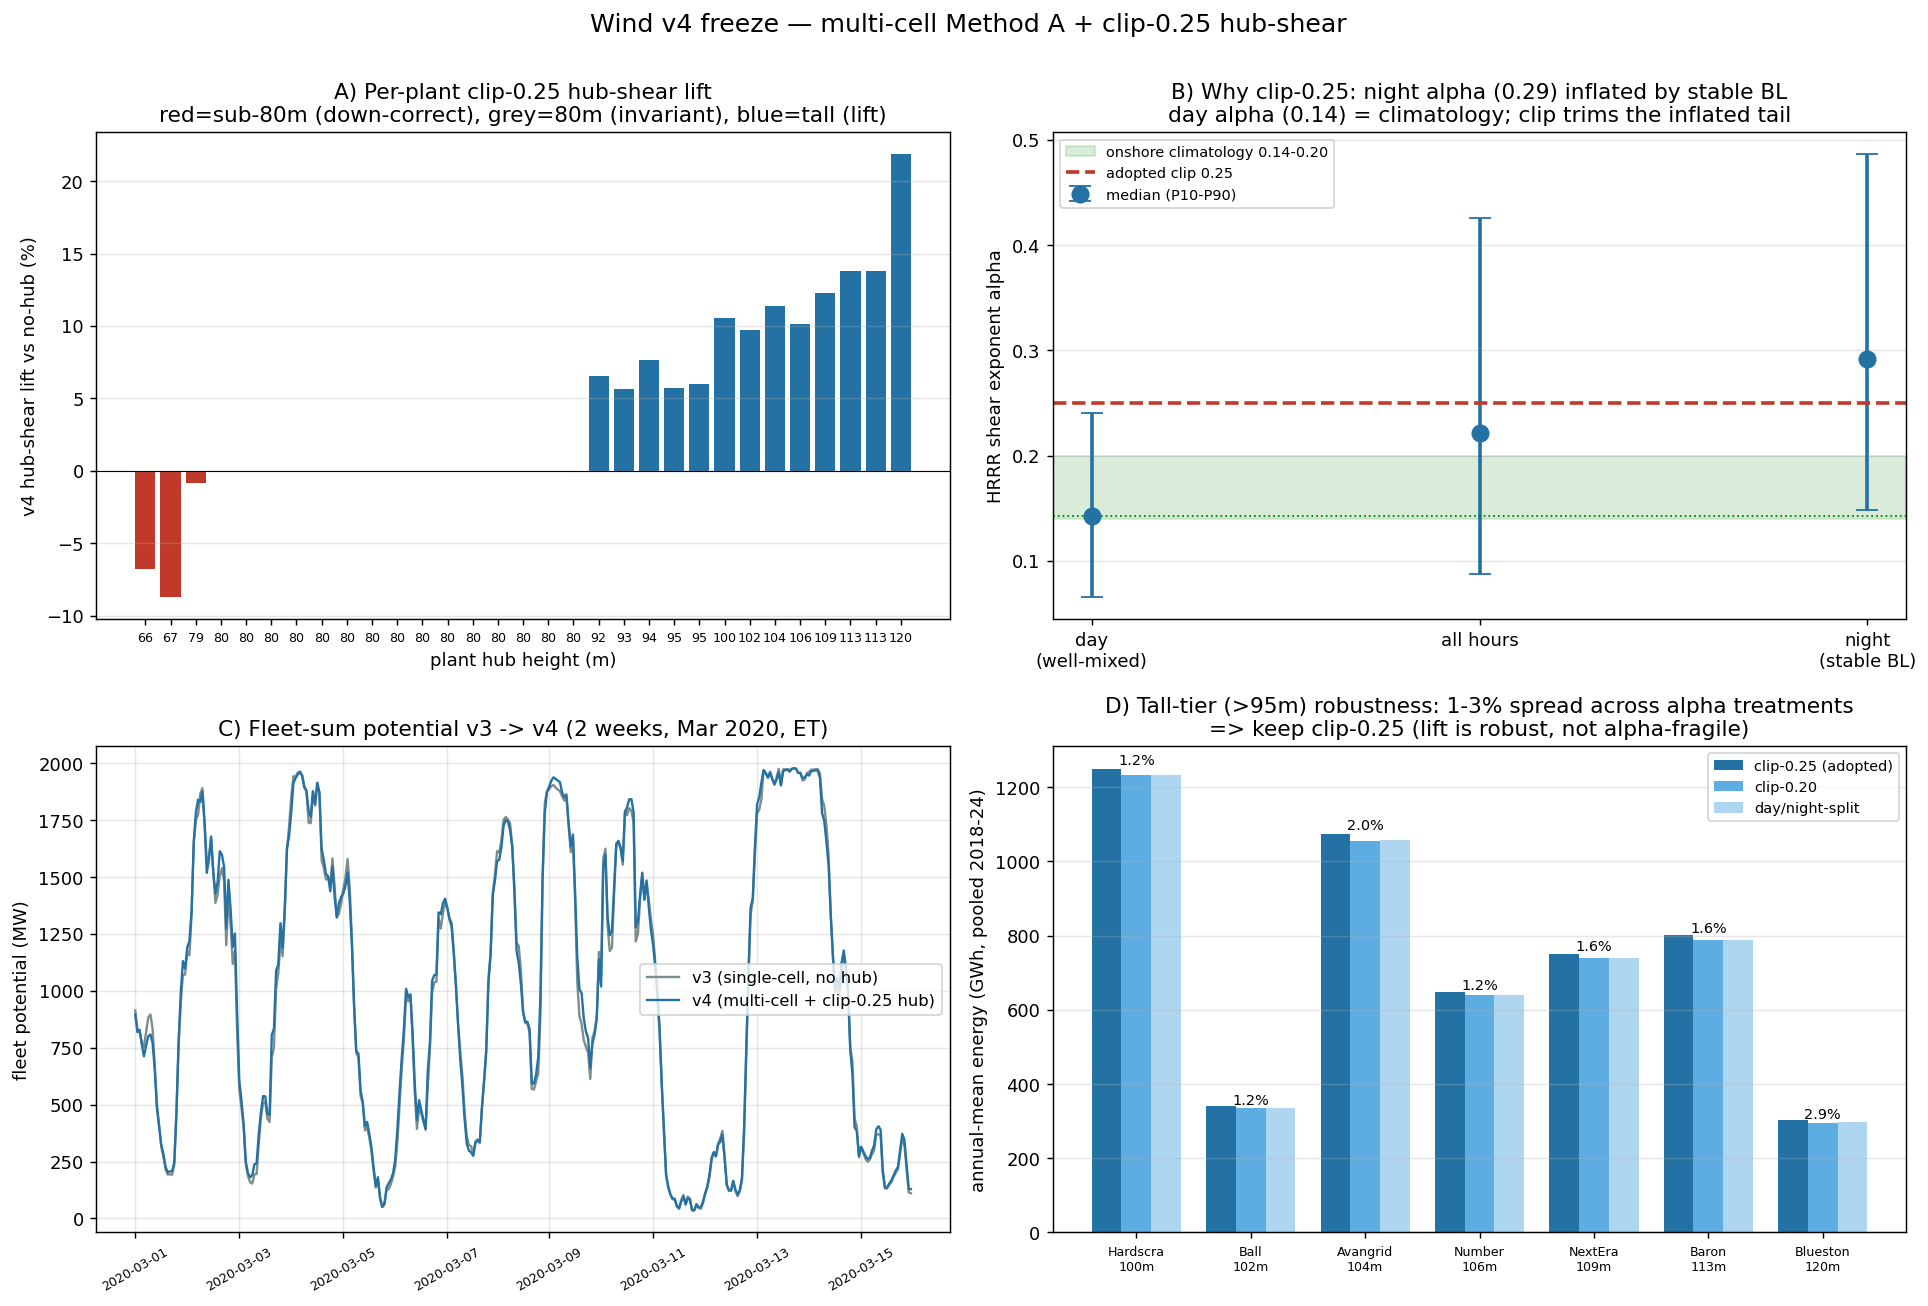
\includegraphics[width=\textwidth]{v4_summary.png}
  \caption{The two extensions to the PLUSWIND recipe.
    (A)~per-plant hub-shear lift against hub height, with the 80\,m
    plants, the two short plants at 66--67\,m, and the tall plants
    distinguished by colour. (B)~the measured shear exponent $\alpha$
    for daytime, all hours, and night-time, with the onshore
    climatology band and the adopted $0.25$ clip marked. (C)~fleet
    potential over two weeks of March 2020 under the single-cell and
    the multi-cell-plus-shear pipelines. (D)~tall-tier annual-mean
    energy under three $\alpha$ treatments, with the percentage spread
    annotated per plant.}
\end{figure}

\subsection{Stage 3: density correction}

Air density depends on pressure and temperature:
\begin{equation}
  \rho \;=\; \frac{P}{R_d \cdot T},
  \qquad R_d = 287.058\ \text{J/(kg$\cdot$K)},
\end{equation}
with $P$ from HRRR's surface pressure and $T$ from HRRR's 2\,m
temperature. NY conditions span $\rho \approx 1.18$\,kg/m$^3$ on a hot
summer afternoon to $\rho \approx 1.34$ on a cold winter morning ---
about a 10--12\,\% swing.

Wind power is proportional to $\rho \, W\!S^3$, so a 10\,\% denser air
on a winter day means 10\,\% more power flowing through the rotor at the
same wind speed. Manufacturer power curves are published at standard sea-
level density $\rho_0 = 1.225$\,kg/m$^3$. The International
Electrotechnical Commission (IEC) standard 61400-12-1 for wind turbine
power performance~\citep{iec614001212017} folds the density correction
into the wind speed instead of the power so
that the manufacturer's curve can be applied unmodified:
\begin{equation}
  W\!S_\text{corrected} \;=\; W\!S \cdot
    \left(\frac{\rho}{\rho_0}\right)^{1/3}.
  \label{eq:density}
\end{equation}
The cube root makes the wind speed correction modest --- a 10\,\% density
swing is a 3.3\,\% wind speed shift --- and the cubic dependence of power
on wind speed inside the curve recovers the 10\,\% in the output.

\subsection{Stage 4: per-plant SAM power curve}

Each plant's power curve is generated once at startup using NREL SAM. We
pass SAM the plant's representative single-turbine specs (mean nameplate
$P_t$ in kW, rotor diameter $D$ in m) and standard reference settings
(maximum power coefficient $C_p^{\max} = 0.45$, drive-train and
tip-speed-ratio defaults, cut-in 3\,m/s, cut-out 25\,m/s). SAM returns a
smooth empirical capacity-factor curve $\mathrm{CF}_\text{SAM}$ on a
0--40\,m/s grid in 0.25\,m/s steps, plus the plant's rated wind speed
$R\!S$ (the speed at which the turbine first reaches nameplate). The same
curve is evaluated independently at every cell the plant occupies, each
cell using its own density-corrected hub-height wind speed.

\begin{figure}[H]
  \centering
  \includegraphics[width=0.85\textwidth]{sam_curve_examples.png}
  \caption{SAM empirical power curves for two NY plants of different
    specific power. Each curve is zero below the 3\,m/s cut-in, rises
    smoothly through the 5--9\,m/s shaded band, and holds at nameplate
    (capacity factor of one) between the rated wind speed and the
    25\,m/s cut-out. The plant's specific power $\sigma$, its rated
    capacity per swept m$^2$ of rotor, sets the steepness of the rise.}
\end{figure}

\subsection{Stage 5: wake/availability loss and aggregation to the plant}

A flat 7\,\% loss accounts for downwind turbines seeing wakes from
upwind ones (typical fleet wake losses average 4--6\,\%) and for plant
availability (turbines down for maintenance, icing, blade damage; another
1--3\,\%). The loss is held flat below rated and tapered to zero above
rated wind speed, on the physical reasoning that once every turbine in
the plant is at nameplate there is no headroom for wake derate:
\begin{equation}
  L(W\!S) \;=\;
  \begin{cases}
    0.07 & W\!S < R\!S - 0.5 \\[4pt]
    0.07 - 0.07\cdot\dfrac{W\!S - (R\!S - 0.5)}{2.5}
      & R\!S - 0.5 \le W\!S \le R\!S + 2.0 \\[10pt]
    0 & W\!S > R\!S + 2.0
  \end{cases}
\end{equation}
The taper width (2.5\,m/s) and the offset (0.5\,m/s below rated) match
PLUSWIND's specification. Because the loss is a function of the
(hub-corrected) wind speed, it is evaluated per cell along with the
curve, so a plant straddling cells of different wind sees a continuous
loss across its footprint rather than a single value at the plant mean.

The plant's potential generation is then the turbine-weighted sum of the
per-cell contributions (Method~A of Stage~1). Writing $w_c$ for the share
of the plant's turbines in cell $c$ and $W\!S_c$ for that cell's
density-corrected hub-height wind speed,
\begin{equation}
  P_\text{plant}^\text{final}
    \;=\; \text{nameplate}_\text{plant} \sum_{c} w_c\,
      \mathrm{CF}_\text{SAM}\!\bigl(W\!S_c\bigr)\,
      \bigl(1 - L(W\!S_c)\bigr),
      \qquad \sum_c w_c = 1.
  \label{eq:final}
\end{equation}
A single-cell plant ($w_c = 1$ for one cell) reduces to the elementary
form $P = \text{nameplate}\cdot\mathrm{CF}\cdot(1-L)$.

\subsection{Day-ahead forecasts: same physics, different HRRR run}

The day-ahead forecast applies stages (1)--(5) unchanged; it differs from
the actuals only in which HRRR file feeds them. The actuals use HRRR's
F00 analysis valid at the target hour --- the model's best estimate of
the atmosphere as it actually was. The forecast uses a single
day-ahead-market issuance: the $18$\,Z cycle of the previous day,
forecast horizons F06--F29, which covers the next calendar day's
$24$ hours. The same Python routine processes both --- it does not know
which kind of HRRR file it has been handed, so any difference between
the two series reflects HRRR's analysis-versus-forecast skill at
day-ahead lead, not the power conversion. The forecast series receives
one further layer of post-processing, a statistical bias correction
described in Section~\ref{sec:forecast}; the actuals do not.

% ============================================================================
\section{Validation}
\label{sec:validation}

Validation proceeds in three layers, each answering a different
question. The first, against PLUSWIND and the subject of this section,
asks whether our implementation of the shared SAM-physics core
reproduces the published reference. This is a model-versus-model check
on the same HRRR inputs, and because PLUSWIND is itself single-cell and
80\,m it is run with our multi-cell and hub-shear extensions disabled,
so the comparison isolates the core. The second, against the clean
Copenhagen metered anchor (Section~\ref{sec:hubshear_validation}), asks
whether the two extensions move the absolute level in the physically
correct direction on a plant where metered delivery is close to
potential; PLUSWIND cannot answer this, being structurally blind to hub
height. The third, against Form EIA-923 delivered generation fleet-wide
(Section~\ref{sec:eia923}), asks whether the absolute level of the
potential series is consistent with what NY wind plants actually
delivered, once curtailment and losses are accounted for. The three
layers establish, in turn, reproducibility, correct-direction
calibration of the extensions, and absolute-level plausibility.

For layer (i) the core output is compared against PLUSWIND for each of
the 22 NY plants present in both datasets, hour by hour, across the
2018--2021 window. Two error metrics enter the discussion. The first is
the
normalised mean absolute error (nMAE), the average of $|f-a|$ divided
by the mean of actuals and expressed as a percentage; this measures
the typical magnitude of an hourly miss in units of average wind
output. The second is the bias-corrected nMAE (BC nMAE), in which the
constant mean bias is subtracted from the differences before averaging.
The bias-corrected variant isolates the part of the error that comes
from shape mismatch --- timing, ramps, the diurnal pattern --- because
constant offsets are removed before scoring. A model can have a low
BC nMAE while still being systematically high or low; only nMAE
penalises that.

\subsection{Hourly scatter, all four years pooled}

\begin{figure}[H]
  \centering
  \includegraphics[width=0.55\textwidth]{scatter_v3_vs_pluswind.png}
  \caption{Hourly fleet-sum potential from the in-house core against
    PLUSWIND, 34\,863 observations over 22 NY plants, 2018--2021. Mean
    bias is near zero, nMAE $1.99$\,\%, and bias-corrected nMAE
    $2.07$\,\%.}
\end{figure}

\subsection{Per-year scorecard}

\begin{table}[h]
\centering
\small
\begin{tabular}{lrrrr}
\toprule
Year & n (h) & bias & nMAE & BC nMAE \\
\midrule
2018 &  8\,595 & $-1.36\%$ & $3.17\%$ & $3.93\%$ \\
2019 &  8\,730 & $-0.07\%$ & $1.65\%$ & $1.66\%$ \\
2020 &  8\,780 & $-0.07\%$ & $1.47\%$ & $1.48\%$ \\
2021 &  8\,758 & $+0.36\%$ & $1.60\%$ & $1.59\%$ \\
\bottomrule
\end{tabular}
\caption{In-house core versus PLUSWIND, fleet-sum bias, nMAE, and
bias-corrected nMAE by year. The elevated 2018 figures coincide with
HRRR's mid-year transition from version~2 to version~3 (July 2018),
discussed in Section~\ref{sec:limits}.}
\end{table}

\subsection{Monthly and diurnal patterns}

\begin{figure}[H]
  \centering
  \includegraphics[width=\textwidth]{monthly_4yr.png}
  \caption{Monthly fleet-mean potential (MW) for the in-house core
    (orange) and PLUSWIND (purple) across the 48 months of
    2018--2021.}
\end{figure}

\begin{figure}[H]
  \centering
  \includegraphics[width=\textwidth]{diurnal_pooled.png}
  \caption{Diurnal pattern for summer (June--July--August, JJA) and
    winter (December--January--February, DJF), pooled across
    2018--2021, for the in-house core and PLUSWIND. Both series peak
    in the overnight hours (US/Eastern).}
\end{figure}

\subsection{Hour-by-hour tracking}

\begin{figure}[H]
  \centering
  \includegraphics[width=0.95\textwidth]{year_zooms_summer.png}
  \caption{The same summer week (July 13--19) of each of the four
    PLUSWIND years, in-house core (orange) and PLUSWIND (purple) at
    hourly resolution.}
\end{figure}

\subsection{Per-plant validation}
\label{sec:per_plant_validation}

The fleet-sum agreement shown above can hide compensating errors at
the plant level: one plant running high can cancel another running
low, so a tight fleet match does not by itself prove that each plant
is well modelled. To check this we computed plant-by-plant nMAE
against PLUSWIND for every NY plant in the 2020--2021 overlap, with
all hours pooled across the two years. The window is restricted to
those two years deliberately: two of the twenty-two PLUSWIND plants
(Steel Winds I, Niagara Wind Power, $20$\,MW, and Erie Wind / Steel
Winds II, $15$\,MW, both in Lackawanna) underwent a turbine repowering
in late 2019 --- Clipper Liberty C93 machines replaced with
GE 2.5-116 machines --- and pooling pre- and post-repowering hours
into a single plant-level comparison would mix two physically different
fleets at those sites. The 2020--2021 window is the largest stretch
of PLUSWIND's coverage in which every NY plant runs on its current
turbines. The result is summarised in
Figure~\ref{fig:per_plant_nmae_pluswind} and the underlying numbers
are written to \code{docs/figures/wind\_v3/per\_plant\_metrics.csv}.

\begin{figure}[H]
  \centering
  \includegraphics[width=0.85\textwidth]{per_plant_nmae_vs_pluswind.png}
  \caption{Per-plant nMAE of the in-house \code{pluswind\_v3} actuals
    against PLUSWIND, 2020--2021 pooled. Each bar is one of the 22
    NY plants present in both datasets, and the dotted vertical line
    marks the across-plant median of $1.1\,\%$.}
  \label{fig:per_plant_nmae_pluswind}
\end{figure}

The across-plant median nMAE is $1.1\,\%$, with three quarters of
the plants below $1.7\,\%$. The distribution has three structural
features worth describing.

The first is the body of the distribution. The seventeen plants at
or below $2\,\%$ nMAE are the bulk of the modern NY wind fleet ---
plants commissioned after 2010 with well-documented turbine specs in
the US Wind Turbine Database. They sit on top of PLUSWIND at the
hour level, which is what one expects from two independent SAM-based
pipelines running on the same HRRR inputs with the same density
correction and the same wake-and-availability loss.

The second is the pair at $7.3\,\%$ nMAE, the two units that share a
single EIA plant identifier (the Maple Ridge / Flat Rock pair noted
in Section~\ref{sec:data}). PLUSWIND publishes one combined number
for the shared EIA, so the pipeline aggregates v3's two NY-unit
columns back to the EIA total before scoring; the residual is
therefore not an artefact of the pro-rata split. Maple Ridge instead
distributes $195$ turbines over roughly $11\,$km of the Tug Hill
plateau at $\sim 600\,$m elevation, the most orographically complex
site in the NY fleet, and both pipelines apply their power conversion
at a single HRRR grid cell at the listed centroid. The residual
concentrates in the 50--250\,MW partial-load output band, where
the steeper section of the SAM curve amplifies the small wind-speed
differences between the two implementations into a few-percent power
disagreement. The bias stays below $1.5\,\%$ in absolute terms and
the fleet sum remains exact.

The third is the two-plant tail at $27\,\%$ and $33\,\%$ nMAE,
visible on the right of the chart. These are the two NY sites that
PLUSWIND models with stale turbine specifications. Steel Winds I
($20$\,MW, commissioned 2007) and Erie Wind / Steel Winds II
($15$\,MW, commissioned 2012) were both repowered in late 2019,
swapping their original Clipper Liberty C93 turbines ($2.5$\,MW,
$93\,$m rotor) for GE 2.5-116 machines ($2.5$\,MW, $116\,$m rotor)
of substantially lower specific power and lower rated wind speed.
USWTDB carries the current GE specifications, and our pipeline
applies a year-aware override in the SAM curve builder
(\code{TURBINE\_SPEC\_OVERRIDES} in \code{wind\_physics.py}) that
switches the two plants between the pre-repowering Clipper and the
post-repowering GE curves at the 2019/2020 boundary. PLUSWIND,
however, was generated from a USWTDB snapshot that predates the
repowering and applies the older Clipper power curve uniformly across
every year it covers, including 2020 and 2021. In the 2020--2021
window shown here the in-house pipeline is therefore on the physically
correct GE curve and PLUSWIND is on its stale Clipper curve, and the
two systematically disagree in the partial-load band --- producing
the elbow visible at the two bottom-row panels of
Figure~\ref{fig:per_plant_scatter}. The absolute MW contribution of
the two plants to the NY fleet is about $9$\,MW combined mean output,
so the fleet-level nMAE is essentially unaffected; the disagreement
is genuine, not a modelling defect.

\begin{figure}[H]
  \centering
  \includegraphics[width=\textwidth]{per_plant_scatter_grid.png}
  \caption{Hourly scatter of in-house \code{pluswind\_v3} against
    PLUSWIND for every plant in the overlap, 2020--2021 pooled, one
    point per plant-hour, panels sorted by nMAE with the lowest
    first. The Maple Ridge / Flat Rock combined panel carries the Tug
    Hill terrain residual discussed above, and the two bottom-row
    plants (Erie Wind, Niagara Wind Power) show the partial-load
    elbow between v3's post-repowering GE curve and PLUSWIND's stale
    Clipper curve.}
  \label{fig:per_plant_scatter}
\end{figure}

The take-away is that for the modern, well-instrumented part of the
fleet --- the part that drives essentially all of the fleet-level
generation --- the per-plant match to PLUSWIND is within roughly two
percent nMAE at the hour level. The fleet-level numbers in
Section~\ref{sec:validation} reflect this, not the cancellation of
larger compensating errors. Two of the residuals in this comparison
are, in fact, the symptoms the extensions of Stages~1--2 are designed
to remove: the Maple Ridge elbow is the single-cell artefact of a
plant that spans $16$\,km of terrain, and any tall plant evaluated here
at $80$\,m carries the height bias that the shear correction addresses.
The next subsection validates those corrections on a reference PLUSWIND
cannot provide.

\subsection{Validating the two extensions: the Copenhagen anchor}
\label{sec:hubshear_validation}

The multi-cell aggregation and the hub-height shear move the model
\emph{away} from PLUSWIND by construction, so PLUSWIND cannot test
whether they move it in the right direction. The level of a potential
series can only be checked against real metered delivery, and only on a
plant clean enough that delivery is close to potential --- i.e.\ a plant
with little curtailment and high availability. Copenhagen Wind ($79.9$
MW, $95$\,m hub, Lewis County, commissioned 2018) is that plant: its
hourly delivered generation, published in NYISO's operator-portal LPI
feed, runs within a few percent of any potential estimate, so it is the
one site where the absolute level is meaningfully checkable.

Against Copenhagen's 2024 metered delivery, the model with the 80\,m,
single-cell treatment sits essentially \emph{at} the metered level
(implied loss near zero), which is unphysical: a real plant always loses
a few percent to availability and wake, so its potential must exceed its
delivery. Turning on the hub-height shear lifts Copenhagen (a 95\,m
plant) by about five percent, placing the potential a physically
sensible $\sim 5\,\%$ \emph{above} delivered --- the expected
availability-plus-wake gap for a clean plant --- while leaving the
hourly shape (correlation, ramp timing) unchanged or slightly improved.
The shear correction thus moves the one checkable plant from an
impossible position to a physical one. This is the empirical basis for
adopting it, and the basis for the $\alpha$ clip ceiling of $0.25$
calibrated in Section~\ref{sec:hubshear}.

\begin{figure}[H]
  \centering
  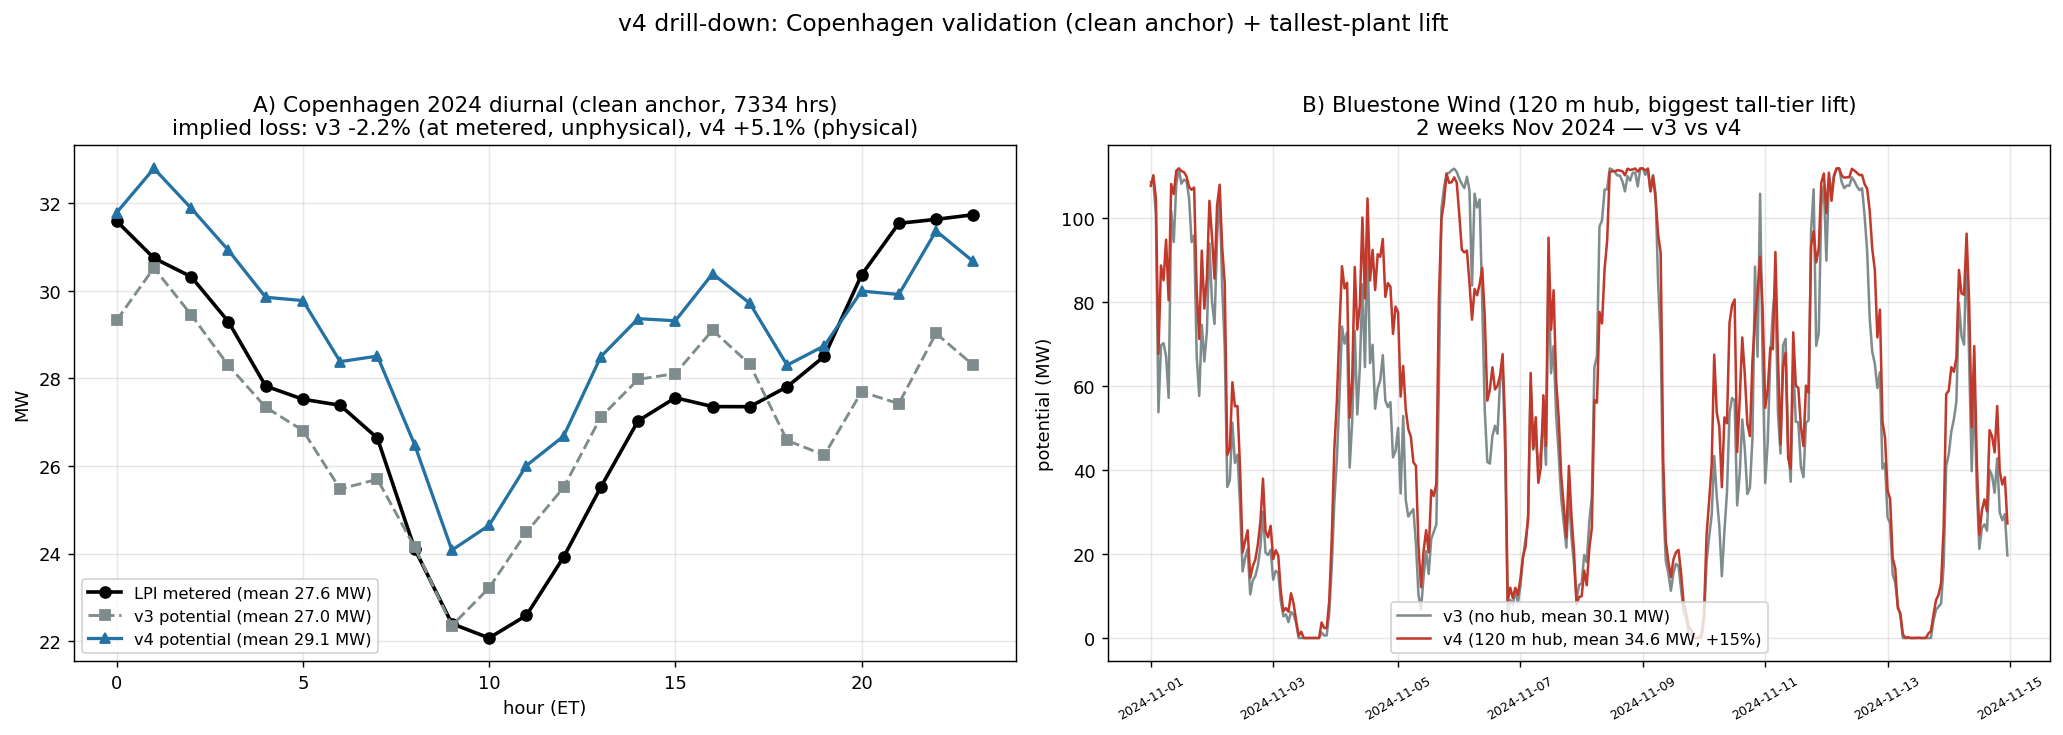
\includegraphics[width=\textwidth]{v4_copenhagen_bluestone.png}
  \caption{Left, Copenhagen 2024 mean diurnal cycle (US/Eastern) for the
    metered LPI delivery and the modelled potential under the $80$\,m and
    the hub-shear treatments. Right, Bluestone ($120$\,m, the tallest
    plant) over two weeks of November 2024 under the single-cell and the
    production series.}
\end{figure}

Copenhagen at $95$\,m is the
tallest plant with a clean anchor. The eight plants above it
($100$--$120$\,m, mostly 2023--2024 commissions such as Bluestone and
Baron Winds) receive larger shear lifts ($+10$ to $+22\,\%$) that
\emph{extrapolate} the power law beyond any ground truth. We bounded the
risk by re-scoring each of these plants under three $\alpha$ treatments
--- the adopted clip at $0.25$, a tighter clip at $0.20$, and a
day/night split that caps the night-time exponent at climatology --- and
found the annual energy of every tall plant stable to within
$1$--$3\,\%$ across the three. The lift is therefore robust to the
$\alpha$ choice, not an artefact of a fragile exponent; what it lacks is
a direct metered check, which only per-resource curtailment data
(Section~\ref{sec:limits}) could supply.

A fleet-wide cross-check comes from NYISO's
real-time fuel-mix feed (\code{rtfuelmix}), which reports statewide
delivered wind at five-minute resolution and is the only independent
signal that touches the whole 2024 fleet, including the tall plants with
no LPI anchor. Summed to the fleet and compared hour by hour across 2024,
the model's potential tracks the shape of statewide delivery closely on
calm and ramping days (Pearson $r$ up to $0.9$), sitting $\sim 25$--$35\,\%$
above it --- the curtailment-plus-availability gap, consistent with the
EIA-923 result below. On the windiest days the shape correlation breaks
down, but in the expected direction: the fleet saturates near rated
while NYISO curtails hard for transmission and economic reasons, so
delivered decouples from potential exactly where a potential model
should not follow it. \code{rtfuelmix} is post-curtailment system total,
so only this shape comparison and a single fleet-level loss scalar are
meaningful from it; it cannot certify per-plant level.

\subsection{Independent cross-check against EIA-923 delivered generation}
\label{sec:eia923}

The PLUSWIND comparison certifies that two independent SAM-based
pipelines agree, but cannot certify the absolute \emph{level} of the
potential series --- both use the same nameplate-based recipe. To
certify the level we add a methodologically independent cross-check
against operator-reported delivered generation from Form EIA-923, the
federally-mandated monthly generation report covering every utility-scale
plant in the United States. The cross-check below was computed on the
single-cell potential series; it transfers directly to the production
multi-cell-plus-hub-shear series, because at the fleet-and-year scale of
this comparison the two differ by well under one percent --- the
tall-plant hub lifts are offset by the Baron nameplate correction and
the sub-80\,m down-corrections (see the metadata paragraph below), so
the fleet-level loss fractions reported here are the production figures.

The model in this document targets \emph{potential} generation: it carries
no curtailment, no outage, and no wake-loss signals beyond the constant
$7\,\%$ factor of Step~4 (Section~\ref{sec:validation}). Section~\ref{sec:limits}
states this plainly and predicts, before any EIA-923 work was done, that
the model output should \emph{exceed} metered NY wind generation by
$20$--$30\,\%$ in aggregate. The EIA-923 cross-check is a test of that
prediction.

The cross-check is computed as follows. For each of the seven years
2018--2024 we sum the
hourly \code{pluswind\_v3} actuals series to monthly per-plant totals
on the US/Eastern calendar (the calendar EIA-923 reports against), join
on EIA plant ID, and compute the per-plant and fleet loss fraction
$L = (M-E)/M$, with $M$ the modeled potential MWh and $E$ the
EIA-923 delivered MWh.\footnote{Pipeline:
\code{PGscen-2nd/scripts/11\_download\_eia923.py} downloads and parses
the annual workbooks; \code{12\_join\_eia923\_to\_pluswind.py} produces
the long-format scorecard at
\code{PGscen-2nd/data/NYISO\_real/eia923/eia923\_vs\_pluswind\_v3\_long.csv};
\code{experiments/wind\_validation/score\_vs\_eia923.py} produces the
fleet and per-plant scorecards under \code{docs/figures/wind\_v3/}.}
Of the $29$ NY wind plants with unique EIA IDs in our metadata, $24$
form the \emph{matched} bucket --- verified EIA-ID, EIA-860 lat/lon
agreement within $5\,$km, no commissioning-month conflicts --- which we
use as the headline. Five plants form an \emph{unverified} bucket
(metadata errors documented below, where the model series is suspect)
and one plant forms a \emph{degraded} bucket (model series is correct,
but the real plant operates below registered nameplate); these are
excluded from the headline and reported separately.

The matched-fleet loss fraction is in the
$22$--$29\,\%$ band in every one of the seven years
(Table~\ref{tab:eia923_fleet}), with no trend across the period and
$\pm 0.1$~pp sensitivity to removal of any single matched plant or to
the inclusion or exclusion of any of the unverified-bucket plants. The
predicted $20$--$30\,\%$ band from Section~\ref{sec:limits} brackets
every observed year. This is the headline of the cross-check.

\begin{table}[h]
\centering
\small
\begin{tabular}{lrrrrrrr}
\toprule
Year & Plants & Mod (TWh) & EIA (TWh) & Gap & Loss & Curt$^\dagger$ & Residual \\
\midrule
2018 & 19 & 4.78 & 3.41 & $40.5\%$ & $28.8\%$ & $1.1\%$ & $27.7\%$ \\
2019 & 19 & 5.04 & 3.89 & $29.6\%$ & $22.8\%$ & $1.6\%$ & $21.2\%$ \\
2020 & 21 & 5.09 & 3.95 & $28.7\%$ & $22.3\%$ & $1.5\%$ & $20.8\%$ \\
2021 & 21 & 4.88 & 3.67 & $33.2\%$ & $24.9\%$ & $2.0\%$ & $22.9\%$ \\
2022 & 23 & 5.80 & 4.12 & $40.7\%$ & $28.9\%$ & $3.4\%$ & $25.5\%$ \\
2023 & 24 & 5.26 & 4.04 & $30.3\%$ & $23.2\%$ & $3.4\%$ & $19.8\%$ \\
2024 & 24 & 6.17 & 4.75 & $29.9\%$ & $23.0\%$ &     -- &     -- \\
\bottomrule
\end{tabular}
\caption{Matched-fleet annual rollup. Loss $=(M-E)/M$ is the modeled
potential expressed as a fraction of its own output relative to
delivered generation. Curt is the NYISO transmission-driven wind
curtailment from NYISO Power Trends 2024 Figure~18
\cite{nyiso2024powertrends}, and Residual is Loss minus Curt. Partial-year
first-months for mid-year-commissioned plants are excluded from both the
modeled and the EIA sums; 2024 curtailment was not yet published when
the table was assembled. $^\dagger$ Transmission and economic
curtailment only.}
\label{tab:eia923_fleet}
\end{table}

A subset sensitivity test confirms the headline
is not sustained by a small number of plants. Removing each of the five
unverified-bucket plants or the one degraded plant individually, or all
six together, moves the pooled $2018$--$2024$ loss fraction by at most
$0.1$~pp; substituting in each unverified plant as if matched moves it
by at most $0.6$~pp. Treating the five unverified plants as matched (the
most aggressive perturbation) gives $28.9\,\%$ loss instead of $24.9\,\%$,
still inside the predicted band. The result is structural.

The curtailment column requires care in interpretation.
The Curt column reports the share of NY wind production curtailed by
NYISO real-time dispatch for transmission and economic reasons, as
published by NYISO. This is the only NY-specific curtailment time series
that is publicly available as a clean annual percentage. It does
\emph{not} include reliability-driven out-of-merit (OOM) commitments
that depress wind output (the 2022 Potomac Economics SOM explicitly
documents this for the North Country load
pocket\,\cite{nyiso2022som}), self-curtailment by operators outside the
NYISO signal, wake losses inside wind farms, or scheduled-maintenance
availability. The Residual column in Table~\ref{tab:eia923_fleet} is
therefore the model's loss fraction minus the transmission component
alone, not the model's loss minus all possible non-model effects.

A full quantitative decomposition of the residual $\sim 20\,\%$ into
its physical contributors --- wake, availability, OOM curtailment, and
any residual model bias --- is not attempted here. NYISO does not
publish an inclusive ``total wind output reduction'' figure, and a
proper decomposition would require per-resource MIS curtailment data,
plant-level availability disclosures, and a wake model calibrated to
NY wind farm layouts. The Potomac Economics 2024 SOM moved further
in this direction by analysing individual generators' compliance with
output limits, but still does not collapse to a single annual number.
We note the result and leave the decomposition for a subsequent
validation layer.

Figure~\ref{fig:eia923_monthly_fleet} shows
the monthly fleet sum of modeled potential and EIA-923 delivered across
the full window. The two series trace the same seasonal envelope, with
the gap between them widening modestly in 2021--2022, consistent with
NYISO's documented curtailment escalation in those years.

\begin{figure}[H]
  \centering
  \includegraphics[width=\textwidth]{eia923_monthly_fleet_ts.png}
  \caption{NY wind fleet monthly generation, matched bucket,
    $2018$--$2024$: \code{pluswind\_v3} modeled potential (orange) and
    EIA-923 delivered (blue) across all 84 months. The shaded gap is the
    combined effect of wake, availability, transmission and
    non-transmission curtailment, and any residual model bias.}
  \label{fig:eia923_monthly_fleet}
\end{figure}

The per-plant annual scatter in Figure~\ref{fig:eia923_scatter} shows
the same picture plant-by-plant: modeled values sit consistently above
the $y=x$ line by a fraction comparable to the fleet number, without
the cluster of large outliers that a localised model bug would produce.

\begin{figure}[H]
  \centering
  \includegraphics[width=\textwidth]{eia923_annual_scatter.png}
  \caption{Per-plant annual modeled versus delivered, matched bucket,
    one panel per year. Point colour scales with plant capacity on a
    logarithmic colourbar, each panel's title reports the year's fleet
    gap and loss fraction, and the dashed line is the $y=x$ no-loss
    reference.}
  \label{fig:eia923_scatter}
\end{figure}

A fleet-wide audit cross-checking the NYISO Gold Book, EIA-860, and
USWTDB for all 31 plants found that the apparent ``location errors'' of
an earlier pass were in fact two distinct metadata bugs of the same
EIA-join class, now fixed, plus a handful of genuine outliers.
\emph{Baron Winds} (EIA $60596$) carried a registered nameplate of
$238.4$\,MW inherited from the Gold Book's planning figure, against an
as-built capacity of $130$\,MW (EIA-860) confirmed by its $32$ USWTDB
turbines; the $1.8\times$ overstatement, not any coordinate error, was
what drove its impossible ``$49$--$140\,\%$ loss.'' Correcting the
nameplate brings its $2024$ loss into the $6\,\%$ band. \emph{Canandaigua
Power Partners} (wind\_323617) had been joined to Baron's EIA $60596$ by
the fuzzy matcher --- they share the town of Cohocton --- instead of to
its true Cohocton Wind Project (EIA $56634$); that mis-join gave it
Baron's $113$\,m turbines and coordinates $10$\,km from the real site.
Re-pointing it to $56634$ restores the correct $80$\,m GE\,2.5-116
turbines and location. Both fixes are sourced from EIA-860/USWTDB, never
tuned to metered. The audit confirmed every other plant's coordinates
lie within a few kilometres of its USWTDB turbine centroid (Maple
Ridge's $3.7$\,km is the centroid of a $16$\,km field and is benign).

Two plants remain genuinely uninformative as level checks. \emph{Stony
Creek / Orangeville} (EIA $58088$) and \emph{Noble Wethersfield} (EIA
$56902$) show sustained loss fractions outside the matched band whose
cause is real curtailment or availability rather than a metadata bug ---
their coordinates verify correct --- and await per-resource data to
decompose. \emph{South Fork Wind} (EIA $65561$, offshore) is correctly
identified in EIA-860 but had not yet reported to EIA-923 for $2024$, an
apparent reporting lag.

One additional plant, \emph{Madison Windpower} (EIA $55769$,
$11.5\,$MW commissioned $2000$), is treated separately. The
\code{pluswind\_v3} series for Madison agrees with PLUSWIND's raw
hourly file within $1\,\%$ in every overlapping year --- the two
models are computing the same physics on the same HRRR inputs at the
correct location. EIA-923 delivered output, however, declines from
$\sim 18\,$GWh/yr in $2018$--$2020$ to $\sim 10\,$GWh/yr in $2021$--$2022$
and $7.5\,$GWh in $2024$, consistent with progressive in-place turbine
degradation that EIA-860 has not yet reflected in the registered
nameplate. Both \code{pluswind\_v3} and PLUSWIND assume the registered
nameplate and so both overstate Madison's delivery by a factor of two
to three in the post-degradation period. This is a known
nameplate-driven-potential-model limitation that affects \emph{any}
such model, not a defect of \code{pluswind\_v3} specifically; it is
material here only because Madison is $0.4\,\%$ of the fleet
nameplate.

Within the matched bucket itself,
five plants run consistently $2$--$15\,\%$ below EIA-923: Steel
Winds~I, Steel Winds~II, Fenner, Munnsville, and Hardscrabble. The
five are geographically distributed across Zones A, C, and E, ruling
out a single local cause. Two of them (Steel Winds~I/II) are the
post-repowering GE 2.5-116 sites for which we apply
\code{TURBINE\_SPEC\_OVERRIDES} (Section~\ref{sec:per_plant_validation});
the magnitudes ($2$--$12\,\%$ low) are comparable to manufacturer
power-curve conservatism and to the cluster's narrowness across
geography, suggesting the SAM curve choice for that turbine is
slightly conservative. The cluster's existence is reassurance that
the matched-bucket headline is not a one-sided over-prediction by the
model: four plants run high (where the metadata is broken, see above)
and five plants run modestly low. Across the fleet the model is not
systematically biased.

The per-plant gap heatmap
(Figure~\ref{fig:eia923_heatmap}) and the multi-panel time series for
the differential-outlier plants
(Figure~\ref{fig:eia923_flagged_panels}) are included as supplementary
diagnostics and are not load-bearing for the headline result.

\begin{figure}[H]
  \centering
  \includegraphics[width=\textwidth]{eia923_per_plant_heatmap.png}
  \caption{Per-plant monthly $(M-E)/E \times 100$ gap across the matched
    bucket, $2018$--$2024$. Rows are plants sorted by pooled mean gap, on
    a diverging colourmap centred on the pooled fleet baseline (dark red
    a large positive gap, dark blue a negative gap). Vertical bands span
    all rows in a given month.}
  \label{fig:eia923_heatmap}
\end{figure}

\begin{figure}[H]
  \centering
  \includegraphics[width=\textwidth]{eia923_flagged_panels.png}
  \caption{Monthly modeled and EIA-923 trajectories for the fifteen
    plants whose annual gap is more than $15$~pp from the matched-fleet
    baseline in at least three of the seven years, spanning the
    modestly-low cluster (modeled below delivered), the sustained-high
    cluster (modeled above delivered), and the metadata-bug plants of
    the unverified bucket. Red crosses mark partial-year months excluded
    from the scorecard sums.}
  \label{fig:eia923_flagged_panels}
\end{figure}

The two cross-checks certify different things. The PLUSWIND
comparison in Section~\ref{sec:validation} certifies that two
independent SAM-based pipelines applied to the same HRRR inputs
produce the same potential-generation series. It cannot certify that
the absolute level of that series is right, because PLUSWIND uses the
same nameplate-based methodology. EIA-923 supplies what PLUSWIND
cannot: an independent absolute level reference against
operator-reported delivered generation, with the published NYISO
transmission curtailment number subtracted to keep the comparison
honest. The two layers together establish both reproducibility and
absolute calibration. They are complementary, not redundant.

% ============================================================================
\section{Day-ahead forecasts}
\label{sec:forecast}

The pipeline produces a day-ahead forecast for every plant and every
hour, alongside the actuals series of Section \ref{sec:validation}.
Where the actuals use the HRRR analysis valid at the target hour ---
the model's best estimate of the atmosphere as it actually was --- the
forecast uses HRRR runs initialised at least a day earlier, so the
information available to it is genuinely a day-ahead view. Both halves
are needed downstream: PGScen learns the distribution of forecast
errors from historical pairs of $(actual,\ forecast)$ values, then
samples from that distribution to populate its scenarios.

\subsection{Construction}

The forecast follows a single day-ahead-market issuance. For each
calendar day, the previous day's $18$\,Z HRRR cycle provides the
forecast for all $24$ hours of the day, at forecast horizons F06 through
F29 --- the extended-range horizons that cover the next day from an
$18$\,Z launch, and that have been archived for the $18$\,Z cycle since
the HRRRv3 transition of July 2018. Each forecast hour is processed
through the identical five-stage chain that produces the actuals
(Section~\ref{sec:model}): the same multi-cell mapping, hub-height
shear, density correction, power curve, and loss. The same routine
processes both series and does not know which kind of HRRR file it has
been handed, so any departure of the forecast from the actual reflects
HRRR's own analysis-versus-forecast skill at day-ahead lead, not the
physics conversion. (One consequence of relying on the $18$\,Z extended
horizons: the afternoon/evening forecast hours of early 2018, before the
HRRRv3 transition, are not in the archive and are absent from the 2018
forecast file; 2019 onward is complete.)

\subsection{Statistical bias correction}

Forecasts produced by the steps above carry a small but persistent
positive bias and a diurnal shape that drifts modestly from the
actuals'. Both behaviours come from HRRR itself at lead times of
24--40 hours, and neither has anything to do with the power conversion;
the same conversion that fits the actuals to PLUSWIND within $\sim
1.5\%$ does not invent these errors. To address them we apply a
plant-conditional Model Output Statistics correction. For each
combination of plant, calendar month, and hour-of-day --- 288 bins per
plant --- four numbers are estimated from the historical pairs of
actual and raw-forecast values: the means $\mu_a$ and $\mu_f$ and the
standard deviations $\sigma_a$ and $\sigma_f$. The corrected forecast
is
\begin{equation}
  f_\text{corrected} \;=\;
    (f_\text{raw} - \mu_f) \cdot \frac{\sigma_a}{\sigma_f} + \mu_a,
  \label{eq:mos}
\end{equation}
to which we then apply a three-hour centred rolling average within
each issued forecast block, to suppress per-hour noise from the
numerical weather prediction (NWP) model, and a clip to the interval
$[0,\ \text{cap}]$ that enforces the plant's physical bounds.

The four parameters in Equation \ref{eq:mos} are estimated on a window
that excludes the year being corrected. For the 2023 series shown
below the fit uses the four prior years 2019--2022; for any other
year the operational rule is the same. This rolling arrangement
mirrors what an operational deployment would do --- the correction
available at any forecast issue time would only have access to data
preceding it --- and the skill numbers reported below therefore have
no in-sample optimism baked in.

\subsection{Skill}

The forecast was evaluated on the full year 2023 (8\,760 hours across
28 active plants, fleet capacity 2\,638\,MW). The headline numbers,
normalised to the fleet nameplate, are summarised in Table
\ref{tab:forecast_skill}. The raw forecast carries a positive bias of
about four and a half percent of capacity and a fleet-mean absolute
error of just over seven percent. The MOS correction removes
approximately two-thirds of the bias and trims about fifteen percent
off the mean absolute error. A rolling-window MOS, fitted only on
2019--2022, is essentially indistinguishable from the in-sample fit
on 2023, both at the level of the bias and at the level of the
absolute error. This is the figure of merit for the rolling-window
hygiene: the year held out from training contributes negligibly to
the fitted parameters, so the operational version of the correction
loses essentially nothing relative to a fit that would have unfair
access to the evaluation year.

\begin{table}[h]
\centering
\small
\begin{tabular}{lrrr}
\toprule
forecast (fleet aggregate) & bias & nMAE & nRMSE \\
\midrule
raw physics                                & $+4.52\%$ & $7.24\%$ & $10.29\%$ \\
in-sample MOS (full pool)                  & $+1.27\%$ & $6.13\%$ & $8.67\%$ \\
rolling-window MOS (2019--2022 fit)        & $+1.30\%$ & $6.15\%$ & $8.74\%$ \\
\bottomrule
\end{tabular}
\caption{Forecast skill on 2023, normalised to the fleet nameplate.
Columns are bias, nMAE, and the normalised root mean square error
(nRMSE, defined analogously to nMAE but with squared rather than
absolute errors). The three rows are the raw physics forecast, the
in-sample MOS fit on the full pool, and the rolling-window MOS fit on
2019--2022; the shipped 2023 forecast is the rolling-window version.}
\label{tab:forecast_skill}
\end{table}

The fleet aggregate hides a wider distribution at the plant level.
Figure~\ref{fig:per_plant_forecast} reports plant-by-plant bias and
nMAE for all twenty-eight active plants in 2023, normalised to plant
nameplate for direct comparison with the fleet line in Table
\ref{tab:forecast_skill}. The across-plant median nMAE is $10.5\,\%$
of nameplate; the spread runs from $7.3\,\%$ on the easiest plant to
$12.9\,\%$ on the hardest, slightly under twice the fleet figure of
$6.15\,\%$. The widening is a textbook spatial-decorrelation effect:
the errors of the twenty-eight partially independent plants average
out at the fleet level by approximately a factor of
$\sqrt{\rho + (1-\rho)/N}$, where $N$ is the fleet size and $\rho$ is
the typical pairwise residual correlation, around $0.3$--$0.5$ for
the New York footprint.

\begin{figure}[H]
  \centering
  \includegraphics[width=\textwidth]{per_plant_forecast_skill_2023.png}
  \caption{Per-plant day-ahead forecast skill in 2023, MOS variant,
    for the twenty-eight active NY plants. Left, bias as a percent of
    plant nameplate; right, nMAE as a percent of plant nameplate,
    ranging from $7.3\,\%$ to $12.9\,\%$ with a median of
    $10.5\,\%$.}
  \label{fig:per_plant_forecast}
\end{figure}

The bias panel on the left shows that the MOS correction succeeds at
the per-plant level too: twenty-five of the twenty-eight plants land
within $\pm 2\,\%$ of nameplate, and the three outliers (Number
Three Wind, Baron Winds, NextEra) sit at roughly $3.5\,\%$. These
three plants commissioned in 2022 or 2023 and therefore enter the
2023 evaluation with only a partial training window of historical
residuals; their larger residual bias is consistent with that. The
nMAE panel shows almost no dependence on plant size --- the
smallest plants ($12$ and $20$\,MW nameplate) and the largest
($238$ and $231$\,MW) sit in the same $8$--$13\,\%$ band, which
suggests that the dominant residual is HRRR forecast error common
across the fleet rather than anything plant-specific.

Because the downstream consumer of the pipeline samples the
per-plant series rather than the aggregate, the per-plant
distribution in Figure~\ref{fig:per_plant_forecast} is the
operational figure of merit, with the fleet-level number serving as
a diagnostic for whether the cross-plant correlations are reasonable.
On a small but consistent margin the rolling-window fit also edges
the in-sample fit at the plant level, with a mean nMAE across plants
of $10.55\,\%$ versus $10.66\,\%$ for the in-sample variant. This is
consistent with the variance-rescaling component of MOS adding noise
rather than signal, which we return to in the next section.

\begin{figure}[H]
  \centering
  \includegraphics[width=0.95\textwidth]{forecast_fleet_2023.png}
  \caption{Fleet aggregate over two representative weeks of 2023, one
    in mid-January and one in mid-July, showing the model actuals
    (black), the raw forecast (red), and the rolling-window MOS
    (blue).}
  \label{fig:forecast_fleet}
\end{figure}

\begin{figure}[H]
  \centering
  \includegraphics[width=\textwidth]{forecast_diurnal_2023.png}
  \caption{Mean diurnal pattern by season for the 2023 fleet, showing
    the actuals, the raw forecast, and the MOS series.}
  \label{fig:forecast_diurnal}
\end{figure}

\begin{figure}[H]
  \centering
  \includegraphics[width=0.95\textwidth]{forecast_scatter_2023.png}
  \caption{Hexbin density of fleet forecast against actual, full year
    2023, with the raw forecast at left and the rolling-window MOS at
    right.}
  \label{fig:forecast_scatter}
\end{figure}

% ============================================================================
\section{Stochastic scenarios}
\label{sec:scenarios}

The actuals and forecasts feed the stochastic scenario engine that is
the immediate consumer of this pipeline. The engine learns the joint
distribution of forecast residuals --- per plant, per forecast horizon,
with cross-plant and cross-horizon covariance --- and emits Monte
Carlo trajectories from which the downstream unit-commitment and
dispatch model samples to plan under uncertainty. Two scenario
constructions were considered during validation. The first is a simple
empirical bootstrap that serves as a sanity check; the second is the
production engine.

\subsection{Two scenario constructions}

The simpler construction is a daily-block bootstrap. For each plant we
collect every complete 24-hour residual sequence $e_d(h) = a_d(h) -
f_d(h)$ from a training window of prior years. For an evaluation day
$D$ we draw $N$ such blocks at random and, hour by hour, add each one
to the forecast for day $D$, clipping the resulting scenario to the
plant's physical bounds. This construction preserves the intra-day
temporal correlation of forecast errors: ramps tend to follow ramps,
calm hours to follow calm hours, because each scenario inherits an
entire 24-hour residual trajectory rather than 24 independent draws.
At the plant level the resulting fan is well calibrated, with the
empirical fraction of actuals falling outside the central P25--P75,
P5--P95, and P1--P99 bands matching the nominal levels (50, 10, and 2
percent respectively) to within half a percentage point on a full year
of evaluation.

The same construction is mildly under-dispersed at the fleet
aggregate, because it does not preserve cross-plant correlation. When
each plant draws its block independently, the fleet sum has the
diversification of an independent ensemble, which is tighter than the
real fleet. A naive variant in which every plant uses the same
training date simultaneously was tested as a possible fix, but it
performs worse rather than better: clipping each plant's residual at
its own nameplate before summing eats more of the variance than the
preserved correlation puts back. Both behaviours are documented in the
validation work, and neither is the production answer.

The production scenarios are produced by the GEMINI engine inside
PGScen. GEMINI is the name of the algorithm at the heart of the
engine, a variant of graphical Least Absolute Shrinkage and Selection
Operator (LASSO) estimation specialised to the separable
asset-by-horizon covariance structure that PGScen needs. The engine
fits a graphical-LASSO precision matrix over Gaussianised forecast
residuals, captures the asset-by-horizon covariance jointly, and then
samples from the resulting Gaussian copula and back-transforms through
each plant's marginal distribution. The scenarios it emits respect
both the per-plant marginals and the cross-plant covariance. This is
the engine the downstream consumer samples.

\subsection{Engine validation}

The engine was run on a seven-day window in 2023, from 15 to 21 July,
generating one thousand scenarios per day from five years of training
history (2018--2022). The fleet-aggregate fan chart in Figure
\ref{fig:scenarios_fan} shows the actual trajectory remaining inside
the P25--P75 band most of the time and never exceeding the P5--P95
envelope on any hour of any day in the window.

\begin{figure}[H]
  \centering
  \includegraphics[width=\textwidth]{scenarios_fleet_fan_7day_2023.png}
  \caption{Fleet-aggregate scenarios over the seven days from 15 to 21
    July 2023, summed across the 28 active plants. The light blue band
    is the P5--P95 envelope of the thousand scenarios at each hour and
    the darker band the P25--P75 envelope, with the actual in black and
    the MOS forecast in solid blue.}
  \label{fig:scenarios_fan}
\end{figure}

For each day of the window we compute the Gneiting--Raftery energy
score,
\begin{equation}
  \mathrm{ES} \;=\; \mathbb{E}\,\lVert X - Y \rVert -
                    \tfrac{1}{2}\,\mathbb{E}\,\lVert X - X' \rVert,
\end{equation}
where $X$ and $X'$ are independent scenario draws and $Y$ is the
realised actual. Per-plant scores normalised to capacity range from
about 27 percent on the calmest day to about 71 percent on the
hardest, and the fleet-mean across the seven days sits in the 27--53
percent band that is typical for HRRR-driven 24-hour scenarios.
Nothing in the distribution of scores points to an anomaly; the
engine is producing scenarios with the expected statistical
properties.

The fleet-aggregate fan is the most visible diagnostic, but the
operational granularity of the engine is per-plant: the
unit-commitment consumer downstream samples each plant's marginal
series, not the fleet sum. Figure~\ref{fig:scenarios_per_plant_panels}
shows twenty random (plant, Eastern-day) panels from 2024, fixed by
random seed for reproducibility. Each panel is one plant on one day,
with $1\,000$ GEMINI scenarios drawn around that day's MOS-corrected
day-ahead forecast. The fan envelopes track the forecast shape
rather than the plant nameplate: on calm days they cluster tight near
zero, on windy days they expand toward the plant cap, and the
realised trajectory (black) sits inside the P5--P95 band on most
hours of every panel and inside the P25--P75 band on roughly half of
them. The panels are not cherry-picked --- the script samples
uniformly from the year and the plant list, then plots whatever it
draws --- so the visual coverage is a fair sample and matches the
calibration numbers from the energy-score distribution above.

\begin{figure}[H]
  \centering
  \includegraphics[width=\textwidth]{wind_random_plant_date_panels_20_2024.png}
  \caption{Twenty random (plant, Eastern-day) panels from 2024,
    seed-fixed for reproducibility. In each panel the light blue
    band is the P1--P99 envelope of $1\,000$ scenarios at each hour;
    the medium band is P5--P95; the dark band is P25--P75; the dark
    line is the median scenario. The black trace with markers is the
    realised actual and the dashed blue trace is the MOS-corrected
    day-ahead forecast. The grey dotted line marks the plant
    nameplate. Plant sizes range from $12$\,MW (Madison Windpower)
    to $238$\,MW (Baron Winds), and the dates span the calendar
    year. Eastern-day windows are stitched from two consecutive UTC
    engine runs so that each panel shows a clean local-time day.}
  \label{fig:scenarios_per_plant_panels}
\end{figure}

\subsection{Open issues}

The 2023 forecast file shipped with the pipeline is the rolling-window
MOS introduced in Section \ref{sec:forecast}. The MOS files for the
remaining years --- 2018, 2019--2022, and 2024 --- were fit in-sample
over the full pool and have not yet been re-fit on the corresponding
rolling windows. The in-sample optimism is small enough that this is
a hygiene improvement rather than a blocker, but it is the natural
next step.

The variance-rescaling component of MOS, the $\sigma_a/\sigma_f$ factor
in Equation \ref{eq:mos}, contributes almost nothing once one moves
out of sample. A bias-only variant that retains only the $\mu_a -
\mu_f$ shift, dropping the variance scaling and the three-hour smooth,
would simplify the correction without losing skill. We did not make
that change here because it would alter the on-disk format consumed
downstream, but it is a candidate cleanup the next time this part of
the pipeline is touched.

The simpler daily-block bootstrap, useful for plant-level intuition
and used in the validation work for that purpose, is calibrated only
at the plant level. Operational fleet-level uncertainty has to come
from the GEMINI engine; the block bootstrap should not be used as a
fleet uncertainty model.

% ============================================================================
\section{Seven-year deliverable}
\label{sec:deliverable}

The model is run for every year 2018 through 2024. For each year, two
files: hourly per-plant actuals and hourly per-plant day-ahead forecasts.
Plants come online during the period and are included from their
operating year onward, so the active fleet grows from 23 plants in 2018
to 31 plants in 2024.

\begin{table}[h]
\centering
\small
\begin{tabular}{rrrr}
\toprule
Year & Active plants & Mean fleet output (MW) & Capacity factor \\
\midrule
2018 & 23 & 698 & 35.3\,\% \\
2019 & 23 & 673 & 34.0\,\% \\
2020 & 23 & 676 & 34.2\,\% \\
2021 & 25 & 688 & 31.5\,\% \\
2022 & 25 & 762 & 34.9\,\% \\
2023 & 28 & 778 & 29.5\,\% \\
2024 & 31 & 972 & 32.5\,\% \\
\bottomrule
\end{tabular}
\caption{Annual fleet-sum mean output and capacity factor by year.}
\end{table}

\begin{figure}[H]
  \centering
  \includegraphics[width=\textwidth]{fleet_7yr.png}
  \caption{Top, monthly fleet output across all seven years (orange)
    with the active nameplate capacity overlaid (grey dashed). Bottom,
    monthly capacity factor.}
\end{figure}

% ============================================================================
\section{Limits and caveats}
\label{sec:limits}

The 2018 series is of slightly lower quality than the later years. HRRR
transitioned from version~2 to version~3 in mid-July 2018, and the first
half of that year has noisier wind components than the rest of the
period; this shows up as nMAE of $\sim$3\,\% against $\sim$1.5\,\% in
subsequent years. PLUSWIND has the same issue.

The model targets potential generation rather than delivered generation.
Because it
contains no curtailment or outage signals, its output can exceed actually
metered wind generation by 20--30\,\% in NY, the curtailment plus
real-world wake and availability loss. For PGScen this is the desired
behaviour; any comparison to NYISO \code{rtfuelmix} or EIA-923 must
expect the model to lie above them, and is a check on shape, not level,
except on the clean Copenhagen anchor
(Section~\ref{sec:hubshear_validation}).

The tall-plant hub lift is validated only indirectly. The
hub-height shear is checked directly against metered delivery only at
Copenhagen ($95$\,m), and the eight plants above $95$\,m extrapolate the
power law beyond that anchor; their lift is robust to the $\alpha$
treatment ($1$--$3\,\%$ spread, Section~\ref{sec:hubshear_validation})
but has no direct ground truth. The single missing piece for a
fleet-wide level validation --- of the hub lift, and of a future learned
power curve --- is per-resource curtailment and availability data, which
NYISO publishes only through its market-information system (MIS).
Acquiring it is the natural next validation layer and would let
\code{potential} $=$ \code{metered} $+$ \code{curtailment} $+$
\code{outage} be reconstructed plant by plant.

Forecast skill is bounded by HRRR's own day-ahead skill. The
day-ahead forecast errors are dominated by intrinsic HRRR forecast
skill at the F06--F29 horizons, not by the power conversion. Improving
forecast quality further would require a different NWP source --- a
blended product such as the National Blend of Models (NBM) or an ECMWF
global forecast --- rather than better physics. The MOS correction
(Section~\ref{sec:forecast}) removes the systematic bias but cannot add
information HRRR did not have.

Per-plant resolution is limited where plants share an EIA identifier.
When two plants in our metadata share an EIA plant identifier (e.g.\
Maple Ridge 1 and 2), they receive the same per-turbine specifications
because USWTDB does not distinguish them; the fleet sum is exact, the
per-plant split approximate. A related, deliberately deferred case is Canandaigua, whose
$125$\,MW is the Cohocton (EIA $56634$) plus Dutch Hill (EIA $56633$)
registrations: its multi-cell footprint currently covers the Cohocton
turbines only, so its level is right (correct curve, hub, nameplate)
while its sub-field ramp variance is slightly overstated. Extending the
cell mapping to span multiple EIA IDs per plant is a fleet-wide
physics-module change held for a later pass.

The day-ahead forecast has incomplete coverage in early 2018. It relies
on the $18$\,Z extended HRRR horizons, which the public archive carries
only from the HRRRv3 transition (July 2018), so the afternoon and
evening forecast hours of January--June 2018 are absent. The actuals
(F00) are unaffected, and 2019 onward is complete.

\appendix
% ============================================================================
\section{Implementation files}
\label{app:files}

The model and the validation tooling live in the project repository. The
production series is the \code{.pluswind\_v4} variant: multi-cell
Method~A with the clip-$0.25$ hub-height shear.

The physics module, \code{PGscen-2nd/pgscen/utils/wind\_physics.py},
contains the SAM curve
builder (\code{build\_sam\_curves}), the density correction, the
wind-shear estimator and hub extrapolation
(\code{estimate\_shear\_alpha}, \code{extrapolate\_to\_hub}, with
\code{SHEAR\_ALPHA\_MAX}\,$=0.25$), the loss model, and the per-hour
power functions \code{pluswind\_v4\_power\_multicell\_A} (multi-cell,
no shear) and \code{pluswind\_v5\_power\_multicell\_A\_hubshear} (the
production path, multi-cell $+$ hub shear). The earlier single-cell
\code{pluswind\_v3\_power\_all\_plants} is retained for the foundation
comparison of Section~\ref{sec:validation}.

The build pipeline runs in two steps under
\code{experiments/wind\_validation/}, because the multi-cell physics
needs the HRRR $80$\,m and $10$\,m winds at every cell a plant occupies.
\code{fetch\_alpha\_raw.py --year YYYY} fetches the six variables at the
union of all fleet cells (one combined byte-range request per hour) and
caches them; \code{build\_v4\_actuals.py} and \code{build\_v4\_forecast.py}
then compute the per-plant actuals (F00) and day-ahead forecasts (the
$18$\,Z F06--F29 issuance) and write them to the \code{.pluswind\_v4}
files.

Forecast bias correction is performed by
\code{PGscen-2nd/scripts/06\_mos\_bias\_correction.py} with
\texttt{--variant .pluswind\_v4}. In-sample mode (\texttt{--years
2018..2024}) fits on the full pool and writes the corrected forecast
back in place after backing up the raw forecast to \code{.raw\_backup};
rolling-window mode (\texttt{--rolling-window 4 --years 2023}) fits on
the four prior years only and writes a sibling
\code{*.pluswind\_v4.rolling.csv}, the operationally honest variant that
produced the 2023 numbers in Section~\ref{sec:forecast}.

Plant metadata lives in
\code{PGscen-2nd/data/NYISO\_real/plant\_metadata/wind\_meta.csv}, the NY
plant table, joined to \code{uswtdb\_ny\_turbines.csv} on EIA plant ID.
The two metadata fixes of Section~\ref{sec:eia923} are enforced by
override guards in \code{scripts/04\_build\_plant\_metadata.py}
(\code{NAMEPLATE\_OVERRIDES} for Baron Winds; \code{EIA\_ID\_COORD\_OVERRIDES}
for Canandaigua) so that a metadata rebuild preserves them.

The output series are
\code{wind\_actual\_1h\_site\_<year>\_utc.pluswind\_v4.csv} and the
matching \code{wind\_day\_ahead\_forecast\_*}, in wide format with one
column per plant. The on-disk index is hourly UTC (the computation
zone); all figures and reported timestamps convert to US/Eastern at the
presentation layer via \code{experiments/wind\_validation/et\_plot.py}.

Validation and figure tooling sits in
\code{experiments/wind\_validation/}, where
\code{score\_per\_plant\_hourly.py} produces
the frozen per-plant scorecard against PLUSWIND, Copenhagen LPI, and the
aged-group LPI, \code{score\_vs\_rtfuelmix.py} the fleet \code{rtfuelmix}
comparison, \code{metadata\_audit.py} the fleet metadata consistency
audit, and \code{analyze\_alpha.py} and
\code{tall\_tier\_alpha\_sensitivity.py}
the $\alpha$ diagnostic and tall-tier sensitivity. The figures in this
document are produced by the \code{make\_*.py} and \code{v4\_*.py}
scripts in the same directory.

The downstream consumers are
\code{experiments/stage\_a\_joint\_load\_wind/} (the joint load-and-wind
Stage~A entry point) and \code{scripts/10\_run\_pgscen\_wind.py} (the
PGScen \code{GeminiEngine} runner), both of which read the
\code{.pluswind\_v4} files.

A local copy of the PLUSWIND methodology PDF lives at
\code{data/pluswind\_docs/PLUSWIND-Documentation.pdf}, and the published
paper is \citet{millstein2023pluswind}.

% ============================================================================
\section{Software dependencies}
\label{app:deps}

\begin{itemize}[leftmargin=*]
  \item \code{nrel-pysam} (PySAM 7.x) --- generates the SAM power curves.
  \item \code{boto3}, \code{botocore} --- anonymous S3 access to NOAA's
        public HRRR bucket.
  \item \code{eccodes} (binary) and \code{cfgrib} --- GRIB2 decoding.
  \item Standard scientific Python: \code{numpy}, \code{pandas},
        \code{scipy}, \code{matplotlib}, \code{tqdm}, \code{xarray}.
\end{itemize}

% ============================================================================
\section*{References}
\label{sec:refs}
\addcontentsline{toc}{section}{References}

\begin{thebibliography}{99}

\bibitem[Blair et~al.(2018)]{blair2018sam}
Blair, N., DiOrio, N., Freeman, J., Gilman, P., Janzou, S., Neises,
T., and Wagner, M. (2018).
\emph{System Advisor Model (SAM) General Description (Version
2017.9.5)}.
Technical Report NREL/TP-6A20-70414, National Renewable Energy
Laboratory, Golden, CO.
\url{https://doi.org/10.2172/1440404}.

\bibitem[Dowell et~al.(2022)]{dowell2022hrrr}
Dowell, D.~C., Alexander, C.~R., James, E.~P., Weygandt, S.~S.,
Benjamin, S.~G., Manikin, G.~S., Smirnova, T.~G., Brown, J.~M.,
Hofmann, R.~J.~P., Smith, M., et~al. (2022).
The High-Resolution Rapid Refresh (HRRR): An hourly updating
convection-allowing forecast model. Part I: Motivation and system
description.
\emph{Weather and Forecasting}, 37(8):1371--1395.
\url{https://doi.org/10.1175/WAF-D-21-0151.1}.

\bibitem[International Electrotechnical
Commission(2017)]{iec614001212017}
International Electrotechnical Commission (2017).
\emph{IEC 61400-12-1:2017 Wind Energy Generation Systems --- Part
12-1: Power Performance Measurements of Electricity Producing Wind
Turbines}.
2nd edition. IEC, Geneva, Switzerland.

\bibitem[Millstein et~al.(2023)]{millstein2023pluswind}
Millstein, D., et~al. (2023).
A database of hourly wind speed and modeled generation for US wind
plants based on three meteorological models.
\emph{Scientific Data}, 10:883.
\url{https://doi.org/10.1038/s41597-023-02804-w}.

\bibitem[NYISO(2024)]{nyiso2024powertrends}
New York Independent System Operator (2024).
\emph{2024 Power Trends: New York's Evolving Electric Grid}.
NYISO, Rensselaer, NY.
Wind generation and curtailment statistics from Figure~18, p.~47.
Archived locally at \code{data/nyiso\_docs/NYISO-Power-Trends-2024.pdf}.

\bibitem[Potomac Economics(2023)]{nyiso2022som}
Potomac Economics (2023).
\emph{2022 State of the Market Report for the New York ISO Markets}.
Independent Market Monitoring Unit, May 2023.
Archived locally at \code{data/nyiso\_docs/NYISO-2022-SOM-Potomac.pdf}.

\bibitem[U.S. EIA(2024)]{eia923}
U.S. Energy Information Administration (2024).
\emph{Form EIA-923: Power Plant Operations Report}.
Annual workbooks 2018--2024.
\url{https://www.eia.gov/electricity/data/eia923/}.

\end{thebibliography}

\end{document}
